\documentclass[11pt]{article}
    %	options include 12pt or 11pt or 10pt
    %	classes include article, report, book, letter, thesis

    \usepackage{amsmath}
    \usepackage{array}
    \setlength\extrarowheight{2pt}
    \usepackage{graphicx}
    \usepackage{epstopdf}
    \usepackage{graphics}
    \graphicspath{ {/home/shanedrafahl/coms331/hw0} }

    \title{HW6}
    \author{Shane Drafahl}
    \date{5 December,2017}

    \begin{document}
    \maketitle

    1. $ \newline $

    a.

    $ \newline $

    \begin{figure}[!htb]
        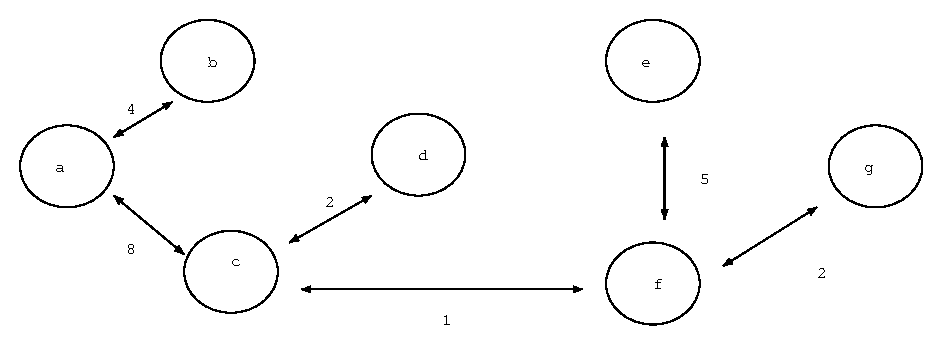
\includegraphics[scale=.7]{./hw5_prim.eps}
    \end{figure}

    $ \newline $

    b. Each vertice has the shortest distance from e listed next to each vertice.

    $ \newline $

    \begin{figure}[!htb]
        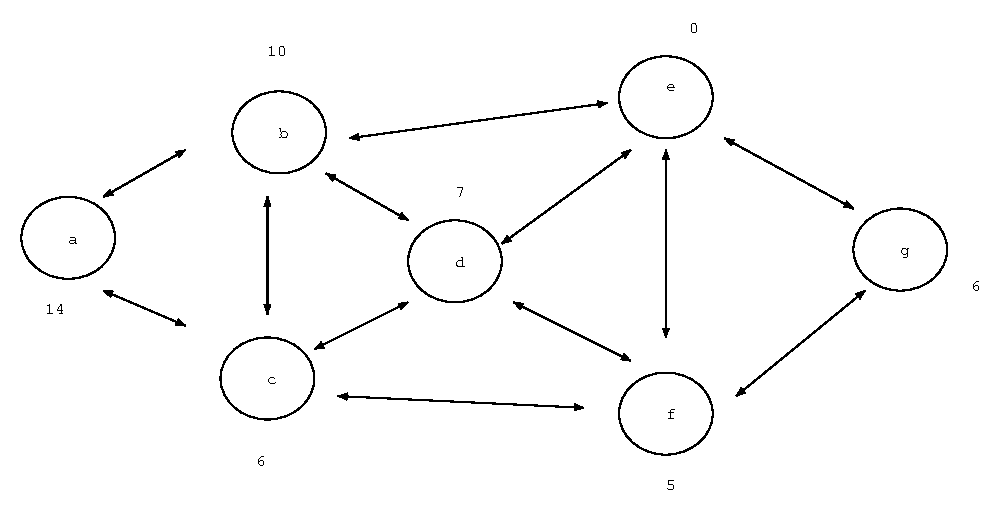
\includegraphics[scale=.7]{./hw5_dyk.eps}
    \end{figure}

    $ \newline $

    2. This algorithm produces a minimum spanning tree. I will prove this by first writing
    a proof to show it will produce a minum spanning tree.

    $ \newline $

    This algorithm starts from the edge with the greatest weight and removes the
    edge if it does not disconect the edge. If we assume by proof of contradiction
    that this algorithm does not produce a tree so it must produce cycles in a graph.
    That means it it cannot remove an edge because it would disconnect the graph.
    This is a contradition because a cycle has more than one path so it should be able
    to remove the edge. Therefore this algorithm will always produce a tree.

    $ \newline $

    Using induction we can prove that the algorithm will produce the minium spanning tree.
    $ \newline $
    Basis: Suppose that there is a set $ F $ of edges currently in the graph. The minimum
    spanning tree must be a subset of $ F $ in the beginning because $ F $ contains all
    edges at this point.
    $ \newline $
    Inductive Hyptothesis: The minimum spanning tree $ T $ is a subset of $ F $.
    $ \newline $
    Induction: We want to show that any edge the algorithm removes by the end of an iteration $ T $,
    the minimum spanding tree, is a subset of $ F $. When the algorithm removes and edge $ c $ we will consider
    the cases.
    $ \newline $
    case 1: $ c \notin T $, for this case $ T $ is still a subset of $ F $.
    $ \newline $
    case 2:  $ c \in T $, for this case removing $ c $ would disconnect $ T $ because $ T $ is a tree.
    The graph must be connected after removing $ c $ so there must exist a cycle before removing $ c $ from $ F $.
    We will call this other cycle not in $ T $ $ f $.
    The algorithm removes the greatest to the smallest weights so we can say that the minimum spaning tree
    is $ T^{''} = T - e + f $ which is a supbset of $ F $. $ T^{'} $ does is a spanning tree because $ e $ is
    removed so the cycle with $ e $ and $ f $ does not exist. The weight of $ e $ equals $ f $ because
    if $ e $ has a greater weight this would be a contradition because $ T $ is a miniumum spanding tree.
    If the opposite were true and $ f $ was greater than $ e $ the algorithm goes throug decending algorithm
    so its impossible for the algorithm to reach two edges that have a cycle with each other and process the
    one with the minium weight. So therefore the weights must equal and thus $ weight(T^{'}) $ = $ weight(T) $.
    Therefore by each iteration the minimum spanding tree is a subset of the remaining edges.
    $ \newline $

    We have proved that each iteration of the algorithm the minimum spanding tree is a subset of the the set of edges
    after each iteration. The minium spanding tree is a subset, so when the algorithm visits all the edges and the loop ends
    the final set of edges should still have the minium spanding tree as a subset. Therefore the final set of edges
    is the minimum spanding tree. Therefore the algorithm produces the minimum spanding tree.

    $ \newline $

    3. In a directed graph, if a vertex can reach all other vertices, then we will call it a
    dominating vertex. Design an algorithm to find the dominating vertices in a graph.
    Prove its correctness and explain the time complexity of your algorithm.

    $ \newline $

    My approach to this problem will be to first convert the graph problem into
    a spanning tree via prims algorithm. This will prevent cycles in the graph.
    Once this is done I can search via DFS from every node in the graph to find
    how many nodes it can find a path to. It will store the max depth it finds
    in each direction for efficiency.

    $ \newline $

    \begin{verbatim}

       G {
            nodes[] // array of Nodes
       }

       N {
            neighbors[] // adjacent nodes
            depth := 1
            searched := false
       }

       algorithm(Graph g) {
            g = primsAlgorithm(g) // creates instance of minimum spanning tree and sets the pointer g to be its pointer
            foreach (Node n in g.nodes) { // iterates over all nodes in the graph
                if(!n.visited) {
                    depth := findDepth(n)
                    if(depth == length(g.nodes)) {
                        return g
                    }
                }
            }
       }

       findDepth(Node n) {
            if(n.visited) {
                return n.distance
            }
            n.visited = true
            foreach (Node n1 in n.neighbors) {
                n.depth += findDepth(n1)
            }
            return n.depth
       }

    \end{verbatim}

    $ \newline $

    First I will prove findDepth. findDepth is a DFS based algorithm.
    For each node it is called uppon changes its value to visited so it cannot
    visit nodes it has visited before. It recursivly finds the depth of each
    adjacent node and sums them together to find the depth. If it has no
    adjacent nodes then it should return one because that is the default. So
    when the algorithm is called on a node that has adjacent nodes that are all
    leaves they would return 1 each meaning its depth would be the number
    of leaf nodes plus one. The plus one being itself. The node that called
    this node then would add that value to its own and its neighbors as well.
    This algorithm cannot get stuck in a cycle either where its depth
    would be in a cycle dependency because prims algorithm is used on the graph
    resulting in a spanning tree that would eliminate any cycles in the graph.
    findDepth is used in the algorithm. The aglorithm visits each node
    that has not been visited and uses findDepth or in other words
    uses DFS on every node to find its depth. If the depth of a single
    nodes equals the number of nodes or the length of the array of nodes
    in the graph that would mean there is a path between that node and every
    other node in the graph.

    $ \newline $

    This algorithm first uses prims algorithm which is $ O(V + E) $. After this
    this is uses a DFS based algorithm on all Nodes that are not visited. I would
    argue this algorithm runs in $ O(V + E) $. Each vertice is only visited once
    in the algorithm. Every Node that is visited by findDepth is marked with
    a visited boolean so it does not need to be processed again. So therefore
    the algorithm grow linearly with its input size. 

    \end{document}
